%%%%%%%%%%%%%%%%%%%%%%%%%%%%%%%%%%%%%%%%%
% DCSE | MITS
% S7 PROJECT PROPOSAL TEMPLATE 
% Version 1.0 (13-08-2017)
% Version 1.1 (03-10-2017)
% Designed by Bineeth Kuriakose, AP, DCSE.
%
%
%
% Each team is free to modify the sections/subsections begins from Rsearch Methodology chapter accourding to the project. 
% But all the chapter headings will remains the same.
% Minimum number of pages required for the project ( the report only, excluding Appendices or reference papers is 30 for Semester 7)
%%%%%%%%%%%%%%%%%%%%%%%%%%%%%%%%%%%%%%%%%
\documentclass[11pt]{report}
\usepackage{graphics}
\usepackage{graphicx}
\usepackage{epsfig}
\usepackage{fancyhdr}
\usepackage{fullpage}
\usepackage{amsmath}
\usepackage{flexisym}
\usepackage{caption}
\usepackage{subcaption}
\usepackage{algpseudocode,algorithm}
\usepackage[section]{placeins}
\usepackage{amssymb} 
\usepackage{textcomp}
\usepackage{tocloft}

\usepackage{setspace}

\onehalfspacing

\newlength{\mylen}
\renewcommand{\cftfigpresnum}{\figurename\enspace}
\renewcommand{\cftfigaftersnum}{:}
\settowidth{\mylen}{\cftfigpresnum\cftfigaftersnum}
\addtolength{\cftfignumwidth}{\mylen}

\renewcommand{\cfttabpresnum}{\tablename\enspace}
\renewcommand{\cfttabaftersnum}{:}
\settowidth{\mylen}{\cfttabpresnum\cfttabaftersnum}
\addtolength{\cfttabnumwidth}{\mylen}


\begin{document}
\renewcommand\bibname{References}
\pagestyle{fancy}
\fancyhead{}
\fancyfoot{}
\fancyfoot[c]{\thepage}
\fancyfoot[l]{\footnotesize B.Tech CSE 2015-19}
%\lhead{abcd}
\renewcommand{\chaptermark}[1]{
\markboth{\thechapter.\ #1}{}} 
\renewcommand{\headrulewidth}{0.1pt}
\fancyhead[r]{\slshape \leftmark}
\addtolength{\headheight}{\baselineskip}
\addtolength{\headsep}{.1in}
\lhead{\nouppercase{\rightmark}}
\rhead{\footnotesize{\nouppercase{\leftmark}}}
\lhead{\footnotesize AYUSH : BLOCKCHAIN BASED HEALTH
RECORD MANAGEMENT SYSTEM} % use any short form if title is lengthy

\begin{titlepage}
\begin{center}

\LARGE{\textbf{AYUSH : BLOCKCHAIN BASED HEALTH
RECORD MANAGEMENT SYSTEM}}\\
\vspace{0.15in}
\large{\textbf{CS451 Seminar and Project Preliminary\\}}
\vspace{1in}

\textit{Project Preliminary Report} \\[0.75cm] 

by\\[0.5cm]
\textsc{\textbf{A V Aswin (University Reg No: MUT15CS002)}}\\[0.25cm] %team member 1
\textsc{\textbf{Basil Reji (University Reg No: MUT15CS018)}}\\[0.25cm] %team member 2
\textsc{\textbf{Basil K Y (University Reg No: MUT15CS019)}}\\[0.25cm] %team member 3
\textsc{\textbf{Vimal P Viswan (University Reg No: MUT15CS058)}}\\[0.25cm] %team member 4

\vspace{1in}
\begin{figure}[h]
\begin{center}

\includegraphics[width=0.7\textwidth]{logo1.png}\\
\end{center}
\end{figure}
\vspace{-0.5cm}
\textsc{Department of Computer Science and Engineering}\\[0.10cm]
%\includegraphics[width=9cm]{mits_logo.jpg}\\
\textsc{\textbf{MUTHOOT INSTITUTE OF TECHNOLOGY AND SCIENCE}}\\[0.10cm]
\textbf{Varikoli P.O, Puthencruz,}\\[0.10cm]
\textbf{Kochi - 682038}\\
\vspace{0.3in}
{\upshape \textbf{November 2018}} % mention the month of your presentation.
\end{center}
\end{titlepage}


%%%%%%%%%%%%%%%%%%%% CERTIFICATE %%%%%%%%%%%%%%%%%%%%%%%
% % % % % % % % % % % % % % % % % % % % % % % % %
\newpage\begin{titlepage}
\center

\textsc{ \textbf{MUTHOOT INSTITUTE OF TECHNOLOGY \& SCIENCE}}\\
\textsc{\textbf{Varikoli P.O, Puthencruz-682308}}
\vspace{0.7cm}
\begin{figure}[H]
\centering

\includegraphics[width=0.7\textwidth]{logo1.png}\\

%\label{logo}
\end{figure}
\vspace{0.2cm}
\textsc{ \small \textbf{ DEPARTMENT OF COMPUTER SCIENCE AND ENGINEERING}}\\




\section*{\centering CERTIFICATE}
%\thispagestyle{empty}
\begin{center}
 This is to certify that this report entitled \textbf{``AYUSH : BLOCKCHAIN BASED HEALTH RECORD MANAGEMENT SYSTEM''} is a bonafied record
of the project work done by \textbf{Mr. A V Aswin (MUT15CS002), Basil Reji(MUT15CS018), Mr. Basil K Y(MUT15CS019), Mr. Vimal P Viswan (MUT15CS058)}under our guidance towards the partial fulfilment of the requirements for the award of Bachelor of Technology in Computer Science and
Engineering of the APJ Abdul Kalam Technological University.
\end{center}
\vspace{1.6cm}

\noindent Guide \hspace{3.5cm} Coordinator\hfill Head of the Department
\\
\noindent Bineeth Kuriakose\hspace{1.62cm}Ms Rakhee M \hfill Dr. Anand Hareendran S\\
\noindent Asst. Professor\hspace{2.05cm} Asst. Professor\hfill Asso. Professor\\
\noindent Dept. of CSE\hspace{2.3cm} Dept. of CSE\hfill Dept. of CSE
%\noindent\textbox{Left longer sample text\hfill}\textbox{\hfil Center\hfil}\textbox{\hfill Right

\end{titlepage}


\newpage

\thispagestyle{empty}


\section*{\centering Acknowledgements}
%\thispagestyle{empty}
\par This project work is the result of our hard work wherein we have been helped and supported by several persons and institutions directly and indirectly. Now it is the time to acknowledge their contributions. 

\par First of all to the Great Almighty, the author of knowledge and wisdom for his countless love. We respect and thank \textbf{Dr.Chikku Abraham}, Vice Principal of MITS for giving us the opportunity to do this project.
With great respect, We express our sincere thanks to our Head of the Department \textbf{Dr. Anand Hareendran} for all the proper guidance and encouragement. I extent my gratitude to the seminar coordinators \textbf{Asst. Prof. Rakhee M}, \textbf{Prof. Dr. Raju.C.K} and \textbf{Asst. Prof. Dr.  Resmi.N.G} for their timely advice, meticulous scrutiny, scholarly advice and scientific approach that helped to a very great extent throughout the seminar. We would like to sincerely thank our guide \textbf{Asst. Prof. Bineeth Kuriakose}, for his support and valuable guidance.

\par We express our heartfelt veneration to all who had been helpful and inspiring throughout this endeavour.
\newline

\noindent\textbf{A V Aswin \\
Basil Reji \\
Basil K Y  \\
Vimal P Viswan}



%%%%%%%%%%%%%%%%%%%% ABSTRACT %%%%%%%%%%%%%%%%%%%%%%%
\newpage
\vspace{2cm}


\begin{abstract}
We are living in a world where data is considered to be the next fuel, also we know how much value the data is. Considering this over the health records which a patient deals with whenever he/ she goes to a hospital, the present scenario lacks a secure  patients health
records to provide more transparency over patients past health data. If the same was available then data sharing between hospitals would have been much easier. In our proposed project, \textbf{Ayush} we are
addressing this problem. We make use of the emerging blockchain technology to achieve this goal.   
\end{abstract}
 
\newpage
\tableofcontents
\newpage
\addcontentsline{toc}{chapter}{List of Figures}

\listoffigures
\newpage

%%%%%%%%%%%%%%%%%%%%%%%%%%%%%%%%%%% INTRODUCTION %%%%%%%%%%%%%%%%%%%%%%%%%%

\chapter {Introduction}  

\pagenumbering{arabic}

At the present scenario we lack a secure database of patients health records to provide more transparency over patient’s past health history. If the same was available then data sharing between hospitals would have been more easier.


\section{Proposed Project}

In our proposed project, we make use of the emerging blockchain technology to achieve this goal. 

\section{Relevance of the Project}

After our project has been successfully completed the problem caused due to handling all the health records involving personal information can be avoided as the patient is the only one having full control over his/her personal information.The transparency issue which existed before over the medical data can also be solved using the emerging Blockchain technology.


%%%%%%%%%%%%%%%%%%%%%% LITERATURE SURVEY %%%%%%%%%%%%%%%%

\chapter{Literature Survey Report}  

\section{Secure Attribute-Based Signature Scheme With Multiple Authorities for Blockchain in Electronic Health Records Systems \cite{1}}
 
\subsection{Summary}
Every patient owns one blockchain of healthcare alone. After being treated in a hospital, all the information including EHRs, consumption records, insurance records, etc. is encapsulated in one block. Patient treatments at different times will be generated in different blocks. Then, a series of blocks are generated according to the time sequence and a healthcare blockchain of patient is constructed.

The rapid development of blockchain technology promotes population healthcare, including medical records as well as patient-related data. This technology provides patients with comprehensive, immutable records, and access to EHRs free from service providers and treatment websites. In this paper, to guarantee the validity of EHRs encapsulated in blockchain, we present an attribute-based signature scheme with multiple authorities, in which a patient endorses a message according to the attribute while disclosing no information other than the evidence that he has attested to it. Furthermore, there are multiple authorities without a trusted single or central one to generate and distribute public/private keys of the patient, which avoids the escrow problem and conforms to the mode of distributed data storage in the blockchain. By sharing the secret pseudorandom function seeds among authorities, this protocol resists collusion attack out of N from N -1 corrupted authorities. Under the assumption of the computational bilinear Diffie-Hellman, we also formally demonstrate that, in terms of the unforgeability and perfect privacy of the attribute-signer, this attribute-based signature scheme is secure in the random oracle model. 


\section{Blockchain: Solving the privacy and research availability tradeoff for EHR data: A new disruptive technology in health data management\cite{2}}

\subsection{Summary}
In  this  paper  they  briefly  introduced  a  new  approach  of  an integrated  health  information  model,  where  a  complex  and  
highly  connected  EHR  can  operate.  The  system  is  based  on  a  newly  discovered  operational  environment,  the  blockchain,  
where  the  heavy  use  of  cryptographic  tools  makes  possible  to build a decentralized and openly extendable network. Elements of  the  solution  are  introduced.  The  new  technology  solves  an  
essential   problem   of   accessing   data   without   endangering   personal privacy. Also, the technology opens new opportunities 
for  automatic  personal  monitoring  devices  and  takes  a  step  
towards involving new service providers as well.  


\section{MedRec: Using Blockchain for Medical Data Access and Permission Management \cite{3}}

\subsection{Summary}
MedRec gives patients a log of their medical history,
which is not only comprehensive, but also accessible and
credible. This restores patient agency, as participants are
now more fully informed of their medical history and any
modifications to it. Through permission management on
the blockchain, we enable patient-initiated data exchange
between medical jurisdictions. To respect the need for confi-
dentiality at a granular scale  MedRec allows for specific
authorizations. Different metadata fields within a
single
record can be shared separately and may include further
restrictions such as an expiration date for viewership rights
(enabled via the smart contract provisions). The blockchain
ledger keeps an auditable history of medical interactions for
patients, providers and regulators.
By integrating with providers’ existing data storage in-
frastructure, medrec facilitate continued use of their existing
systems.


\section{Blockchain: Opportunities for Health Care by Deloitte\cite{6}}

\subsection{Summary}
This paper discuss possibilities of application of blockchain in various healthcare areas.
In the first use, organizations may consider 
blockchain technology to verify a patient’s 
digital identity, genetics data, or 
prescriptions history. Prescrypt, a 
proof-of-concept developed by Deloitte 
Netherlands, in collaboration with SNS Bank 
and Radboud3
, gives patients complete 
ownership of their medical records, allowing 
them to grant and revoke provider access to 
their data. Providers, in turn, can issue 
prescriptions on the blockchain. In the 
second application, organizations can use 
the technology to transfer value, such as 
cryptocurrencies or intellectual property 
rights. Deloitte, in collaboration with Loyyal, 
developed a prototype that incentivizes 
desired behaviors using gamification and 
behavioral economics principles. In the 
future, health ecosystems may emerge 
where providers, plans, or fitness centers 
co-develop programs to incentivize and 
reward patients for healthy behaviors.  
In the third stage of the blockchain 
framework decision making process, 
organizations have an opportunity to 
strengthen
 the system through smart 
contracts that automatically execute when 
conditions are met. This application is 
increasingly sophisticated, using algorithms 
to fully customize conditions that determine 
when to exchange value, transfer 
information, or trigger events. This serves as 
the foundation for more sophisticated 
applications of blockchain technology in 
health care, including prior-authorizations 
and auto-claims processing.
Finally, to 
implement
 a blockchain solution, 
organizations may choose to use a 
permissionless blockchain, such as the 
Bitcoin blockchain, or a permissioned 
blockchain that restricts access to a 
pre-determined group. Consortia such as R3 
in the financial services industry are 
experimenting with permissioned 
blockchains, and R3 has recently completed 
a successful transfer of commercial paper 
between banks
\section{Decentralizing Privacy: Using Blockchain to Protect Personal Data\cite{4}}

\subsection{Summary}
Personal data, and sensitive data in general, should not be
trusted in the hands of third-parties, where they are suscep-
tible to attacks and misuse. Instead, users should own and
control their data without compromising security or limiting
companies’ and authorities’ ability to provide personalized
services. This paper discuss about a platform that  enables this by combining a blockchain,
re-purposed as an access-control moderator, with an off-
blockchain storage solution. Users are not required to trust
any third-party and are always aware of the data that is
being collected about them and how it is used. In addition,
the blockchain recognizes the users as the owners of their
personal data. Companies, in turn, can focus on utilizing data
without being overly concerned about properly securing and
compartmentalizing them.
Furthermore, with a decentralized platform, making legal
and regulatory decisions about collecting, storing and sharing
sensitive data should be simpler. Moreover, laws and regula-
tions could be programmed into the blockchain itself, so that
they are enforced automatically. In other situations, the ledger
can act as legal evidence for accessing (or storing) data, since
it is (computationally) tamper-proof


\section{Securing Mobile Health Data Transmissions with Blockchain Technology\cite{5}}

\subsection{Summary}
Personal health data collected from mobile and wearable technology can provide important information to healthcare providers and medical researchers, but this data must be protected to ensure the privacy of users.
In the blockchain-based system created by the research team, wearable devices collect personal health data, such as physical activity, heartbeat and sleeping conditions from users. Data is then transmitted to a cloud database hosted on a secure platform through a mobile application. To protect privacy, users can manage all personal health data and are responsible for designating the level of access healthcare providers and other third parties have to the cloud server.\par

The blockchain network is connected to the cloud database, and the network records all data updates and requests in the cloud. The researchers used a blockchain network built on the Hyperledger Fabric, which is an open source blockchain with control access designations that certify any participating devices in the network.

To facilitate scalable and efficient data processing and authentication, the researchers developed a Merkle tree-based method for organizing health records in the blockchain. The Merkle method orders submitted data by the time of submission, and then organizes data for simpler management.


\section{Blockchain technology in healthcare: The revolution starts here\cite{7}}
\subsection{Summary}
This paper discuss about
numerous opportunities for usage in the healthcare sector, e.g. 
in  public  health  management,  user-oriented  medical  research  
based on personal patient data as well as drug counterfeiting.  
The   immense   potential   of   this   technology   shows   up   
wherever,  until  now,  a  trusted  third  part
y  was  necessary  for  the  settlement  of  market  services.  With  Blockchain,  direct  
transactions  suddenly  become
  possible,  whereby  a  central  
actor,  who  controlled  the  data,  earned  commission  or  even  
intervened in a censoring fashion, can be eliminated. 
This    disruptive    character,    which    underlies    Blockchain    
technology,  will  strongly  affect  
the  balance  of  power  between  
existing market players in health
care. It will also promote new 
digital business models and digital health initiatives. Due to the 
fact  that,  in  the  future,  (data)  intermediaries  can  be  avoided,  
this  technology  opens  new  doors  with  respect  to  how  market  
interactions  in  healthcare  can  
be  conducted.  Blockchain  thus  
has   an   immense   potential   for   the   future   and   will   show   
disruptive changes in th
e healthcare industry. 
%%%%%%%%%%%%%%%%%%%%%%% PROJECT DESCRIPTION %%%%%%%%%%%%%%%

\chapter {Proposed Work} 


\section{Objectives}  %identify main objectives of your project.

The main objectives of the proposed project are:

\begin{itemize}
        \item To provide a solution for existing issues in health record management systems of hospitals by applying the latest blockchain technology and to have effective and easier sharing of health records between various providers exists .
        \item To design a system in which the patient  have the full control on his health data.
  
        \item To implement a system which will prevent multiple fragmented health records and data loss at different providers.
        \item To design a system which can be used for research purposes with the aid of anonymous health data.
    
    \end{itemize}



\section{Proposed Solution} 

In the proposed system, we are applying  the emerging blockchain technology in for creating transparent health record chain. The platform we are designing will be patient centric and anyone can join the network using an unique identification string like Aadhaar. When someone joins the network, a new block is created for the individual and upcoming events related to this patient will follow this block. When the patient goes to a new hospital, he opts the data to be shared to the new hospital. If any new health data is produced at the new hospital, hospital first adds the information into the IPFS file system. The hash of this file is added to the patient's chain.
\\	The proposed solution is a patient centric one, that is the patient has got the power to give access to his data. The system requires a permissioned network, so we have planned to build this system using a permissioned blockchain. After the literature review and cases study analysis we decided to use the Hyperledger fabric as the tool for our proposed system.
%%%%%%%%%%%%%%%%%%%%%%% SCHEDULING %%%%%%%%%%%%%%%
\chapter{Project Design}
\section{Block Diagram}
    \begin{figure}[h!]
        \centering
        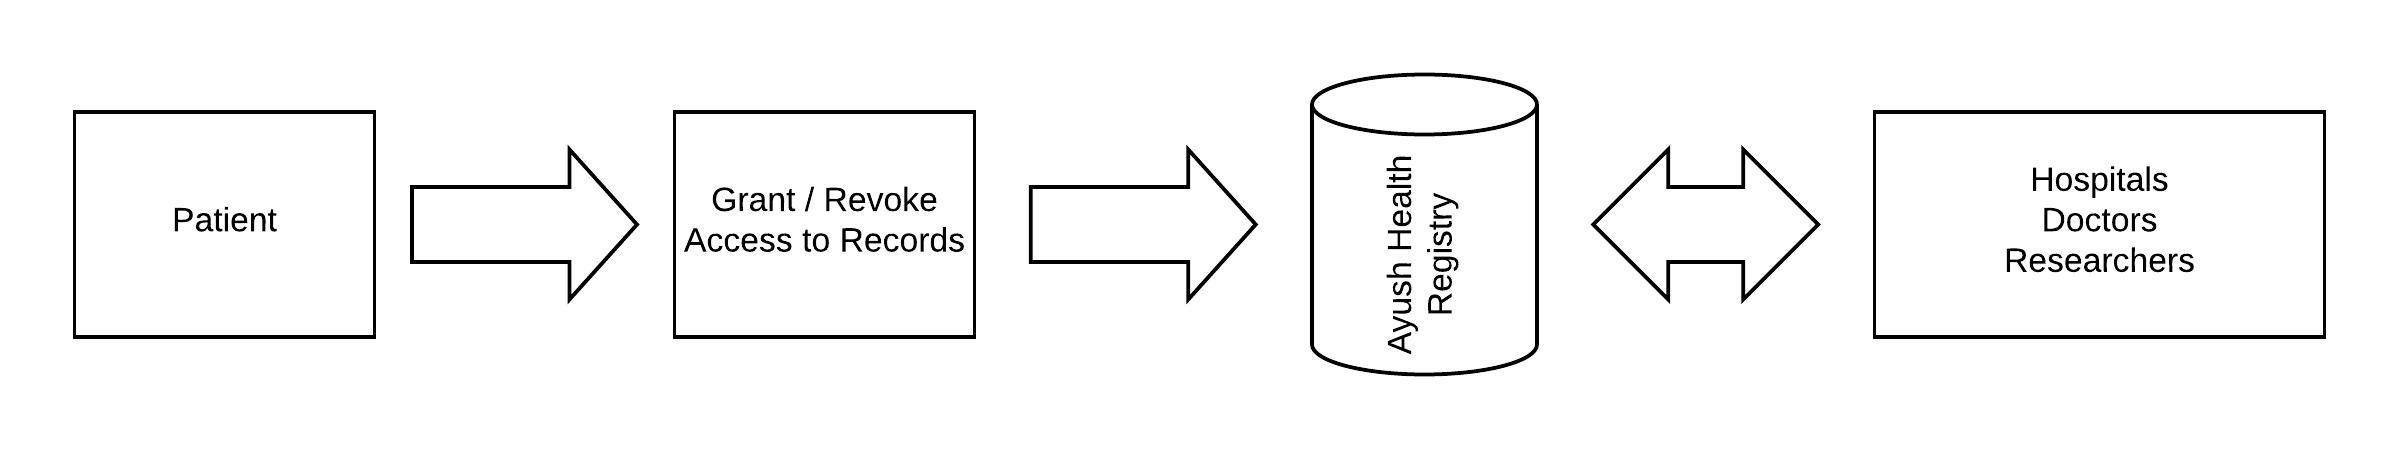
\includegraphics[scale=0.8]{Block.jpeg}
        \caption{Block Diagram}
        \label{fig:my_label}
    \end{figure}
    \newpage
\section{Architecture}        
\begin{figure}[h!]
        \centering
        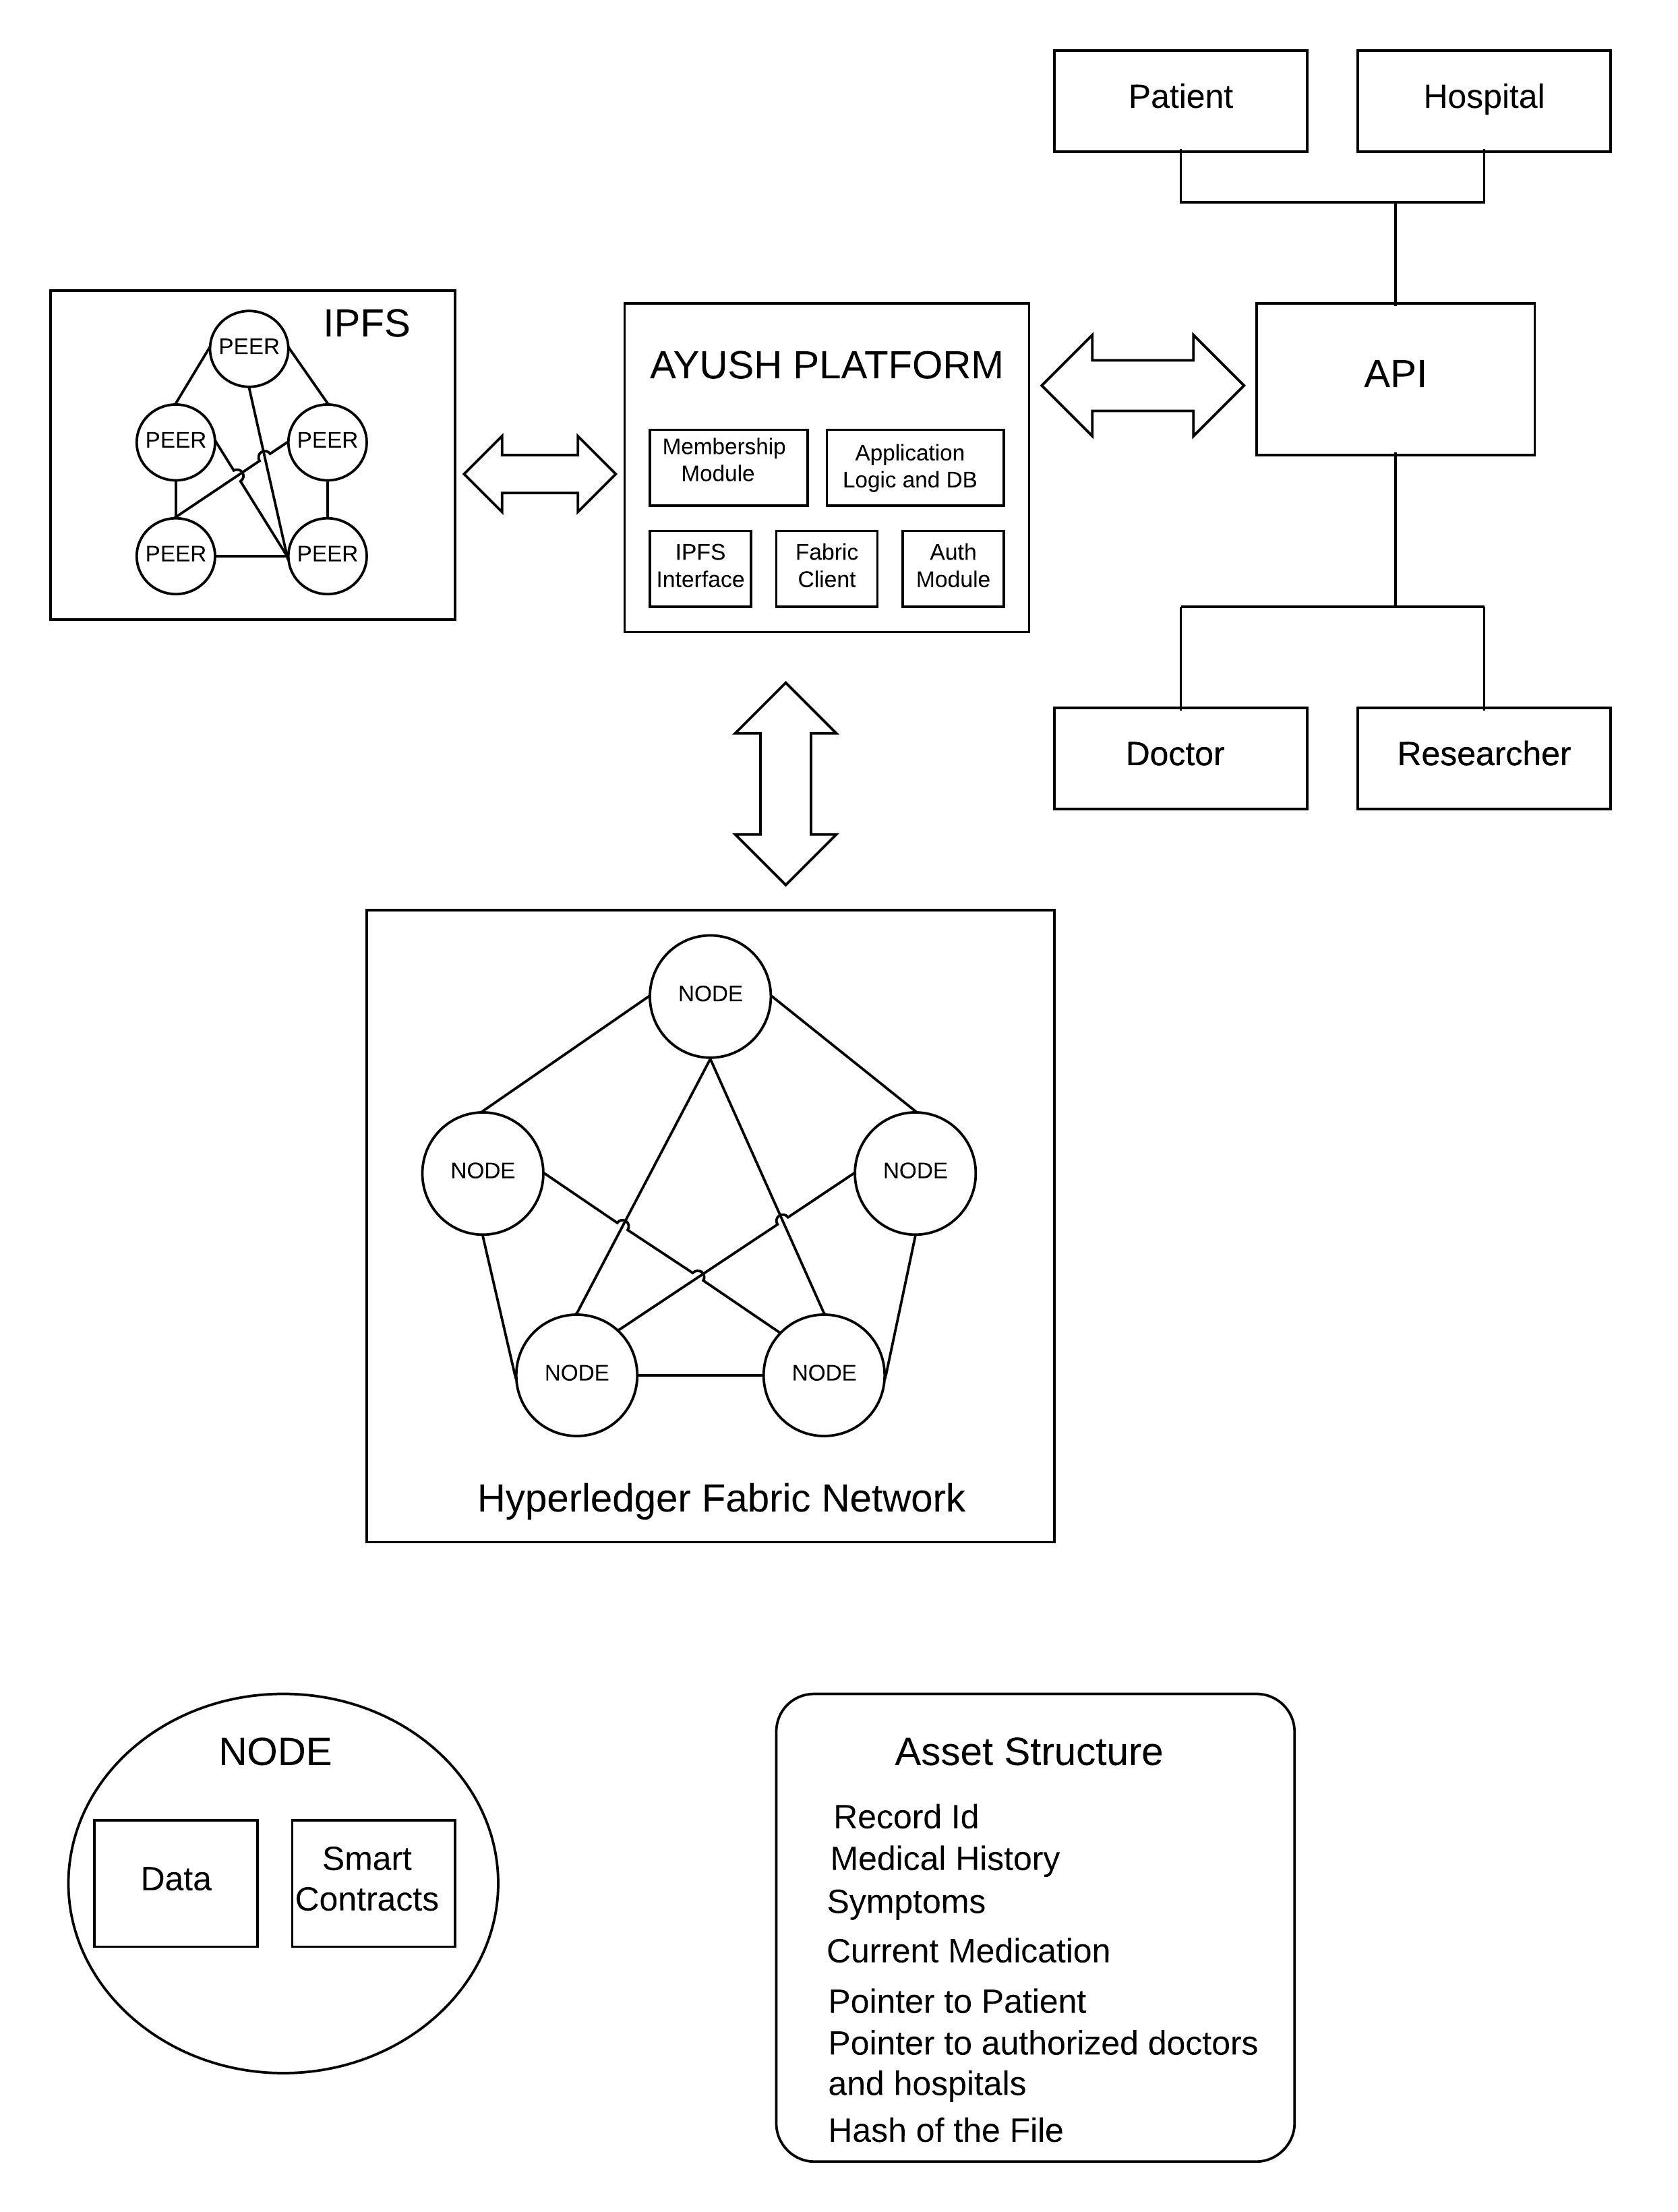
\includegraphics[scale=0.7]{arch.jpeg}
        \caption{Architecture}
        \label{fig:my_label}
    \end{figure} 
Our project mainly have 4 modules :
\begin{enumerate}
    \item API Module
    \item Ayush Platform Module
    \item Hyperledger Fabric Network
    \item Inter Planetary File System (IPFS) 
\end{enumerate}
\subsection{API Module}
API Module act as an interface between Ayush Platform and End Users (Patients, Hospitals and Doctors).It abstracts implementation details of Ayush Platform and Users can interact using simple UI and http requests. 



\subsection{Ayush Platform}
Ayush Platform abstracts implementation details of Hyperledger Fabric, IPFS and provides services to API module. Various modules present in Ayush Network are :
\begin{enumerate}
    \item Fabric Client
    \item IPFS Interface
    \item Auth Module
    \item Membership Module
    \item Application Logic and Database
\end{enumerate}

\subsubsection{Fabric Client}
Fabric Cient encapsulates the APIs to interact with Peers and Orderers of the Fabric network to install and instantiate chaincodes, send transaction invocations and perform chaincode queries.

\subsubsection{IPFS Interface}
Inter Planetary File System (IPFS) Interface is used to communicate with IPFS to upload or fetch from IPFS network.
\subsubsection{Auth Module}
Auth Module is used to recognize a user's identity and allowing only legimate users to interact with the platform.

\subsubsection{Membership Module}
Membership Module is a component that aims to offer an abstraction of a membership operation architecture. In particular, it abstracts away all cryptographic mechanisms and protocols behind issuing and validating certificates, and user authentication. it issues certificates which are used by peers to join the Hyperledger Fabric Network.

\subsubsection{Application Logic and Database}
This module will be responsible for overall operation of the platform and it has a local database also.

\subsection{Hyperledger Fabric Network}
Hyperledger Fabric is a platform for distributed ledger solutions underpinned by a modular architecture delivering high degrees of confidentiality, resiliency, flexibility, and scalability. It is designed to support pluggable implementations of different components and accommodate the complexity and intricacies that exist across the economic ecosystem.Hyperledger Fabric also offers the ability to create channels, allowing a group of participants to create a separate ledger of transactions. This is an especially important option for networks where some participants might be competitors and not want every transaction they make — a special price they’re offering to some participants and not others, for example — known to every participant. If two participants form a channel, then those participants — and no others — have copies of the ledger for that channel.
\par Hyperledger Fabric has a ledger subsystem comprising two components: the world state and the transaction log. Each participant has a copy of the ledger to every Hyperledger Fabric network they belong to.

\subsection{Inter Planetary File System (IPFS) }
IPFS (the InterPlanetary File System) is a new hypermedia distribution protocol, addressed by content and identities. IPFS enables the creation of completely distributed applications. It aims to make the web faster, safer, and more open.
\par IPFS is a distributed file system that seeks to connect all computing devices with the same system of files. In some ways, this is similar to the original aims of the Web, but IPFS is actually more similar to a single bittorrent swarm exchanging git objects. You can read more about its origins in the paper IPFS - Content Addressed, Versioned, P2P File System.





\newpage
\section{Data Flow Diagrams}
    \begin{figure}[h!]
        \centering
        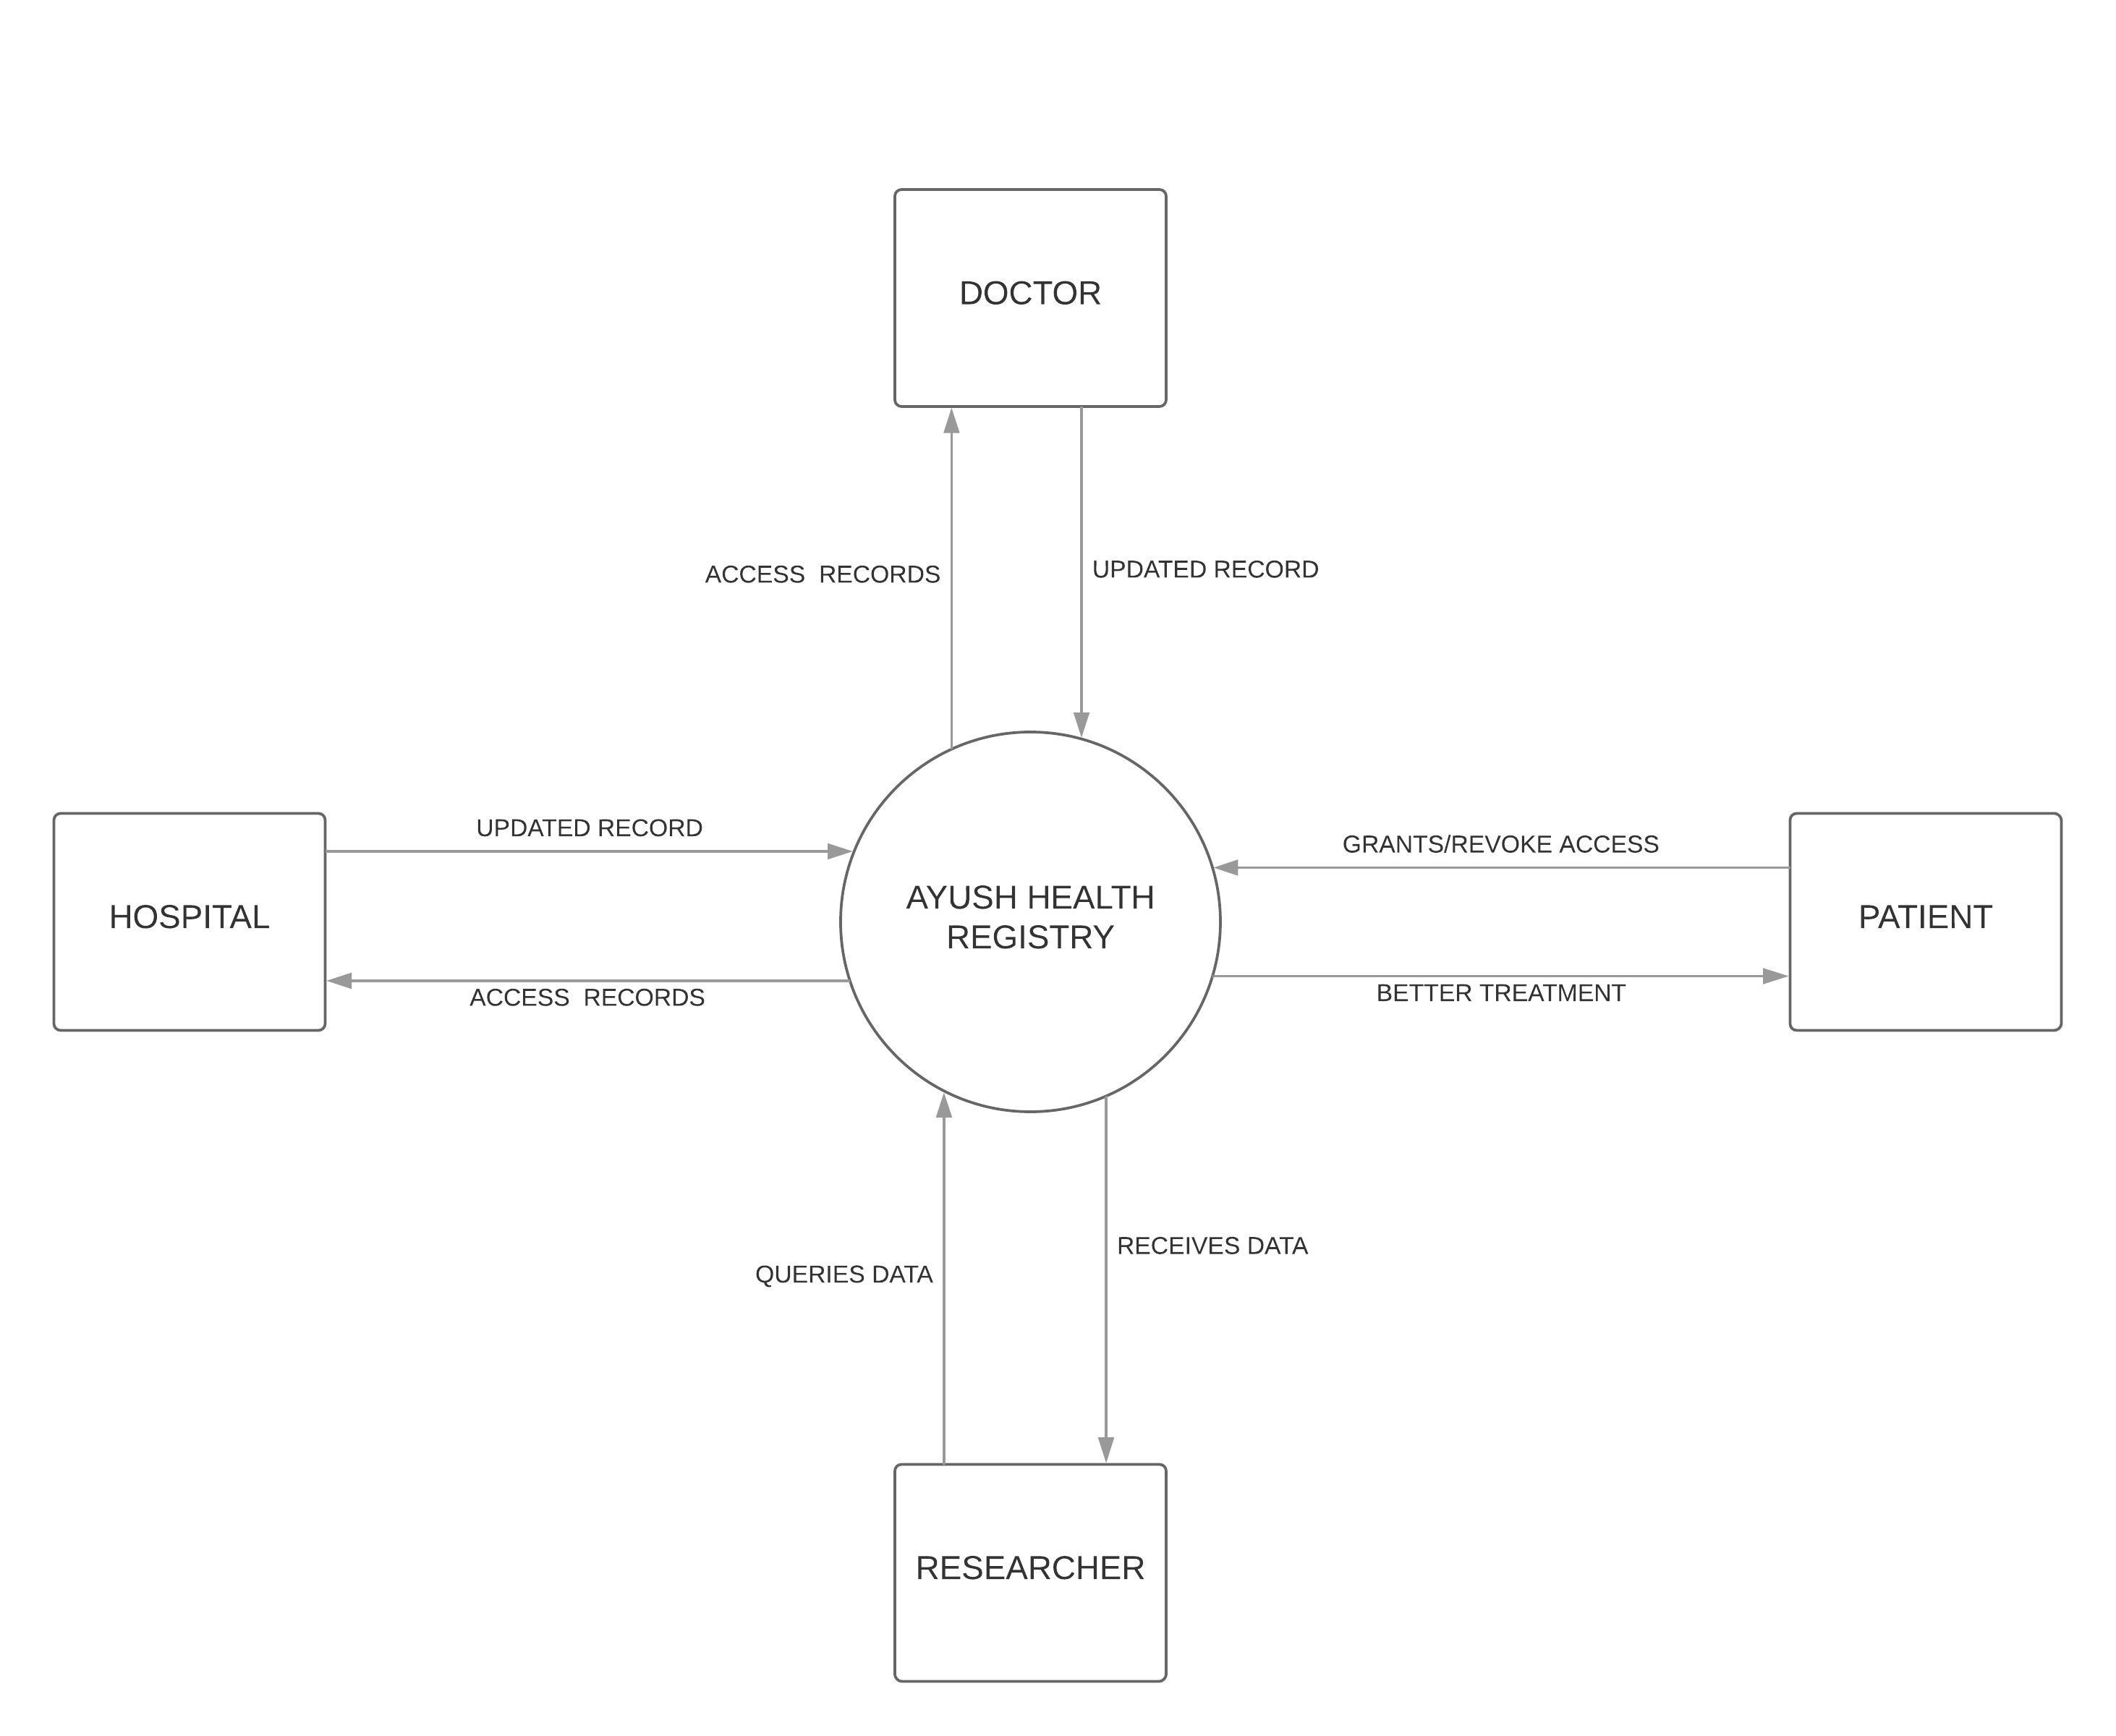
\includegraphics[scale=0.6]{DFD0.jpeg}
        \caption{Level 0 DFD}
        \label{fig:my_label}
    \end{figure}
    \begin{figure}[h!]
        \centering
        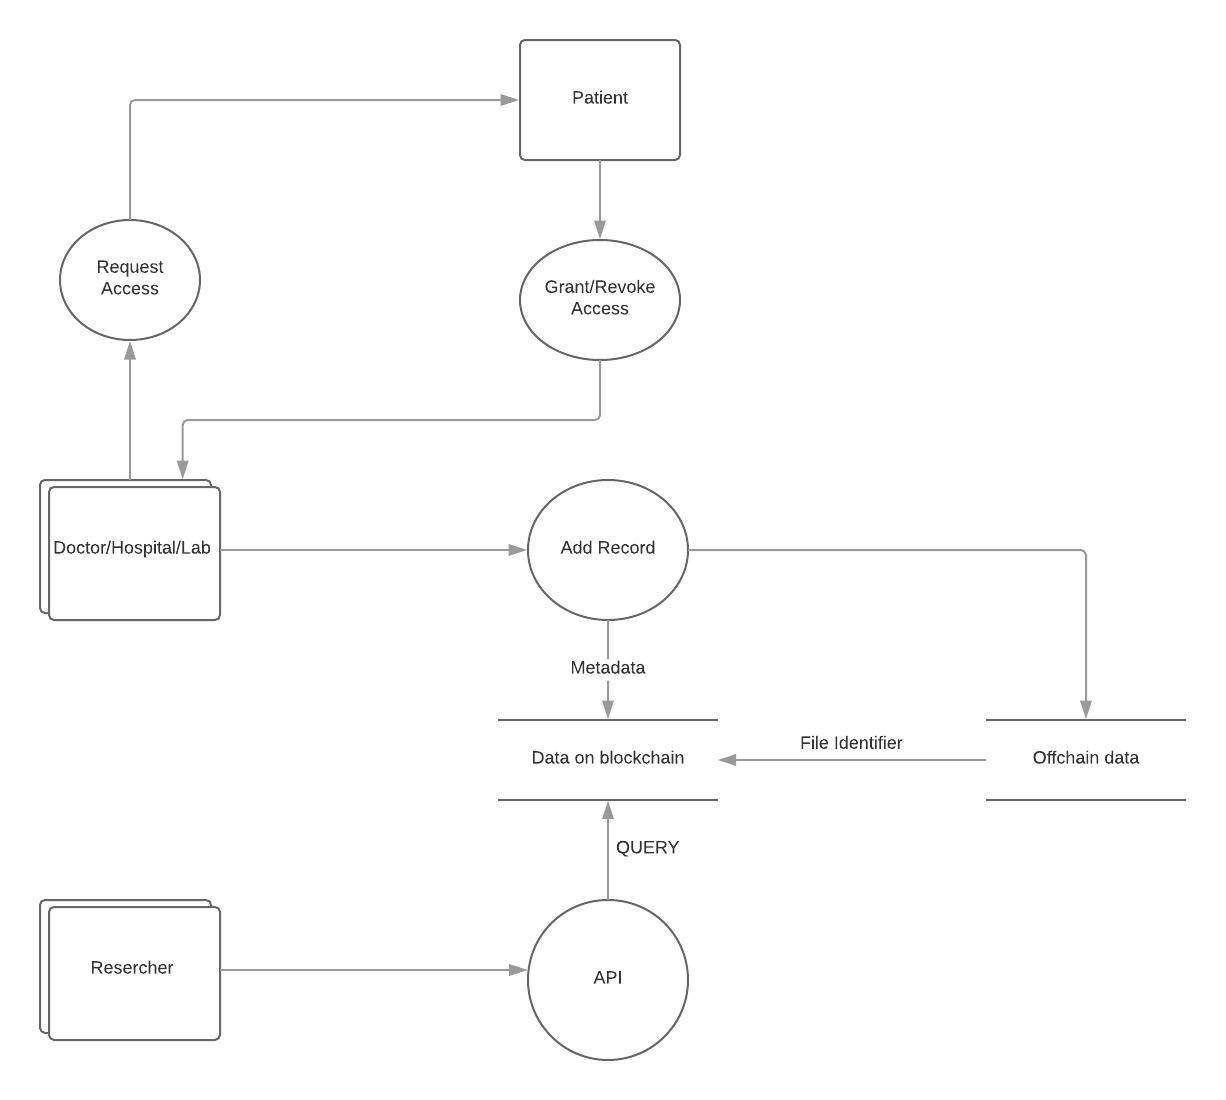
\includegraphics[scale=0.9]{DFD1.jpg}
        \caption{Level 1 DFD}
        \label{fig:my_label}
    \end{figure}
    \begin{figure}[h!]
        \centering
        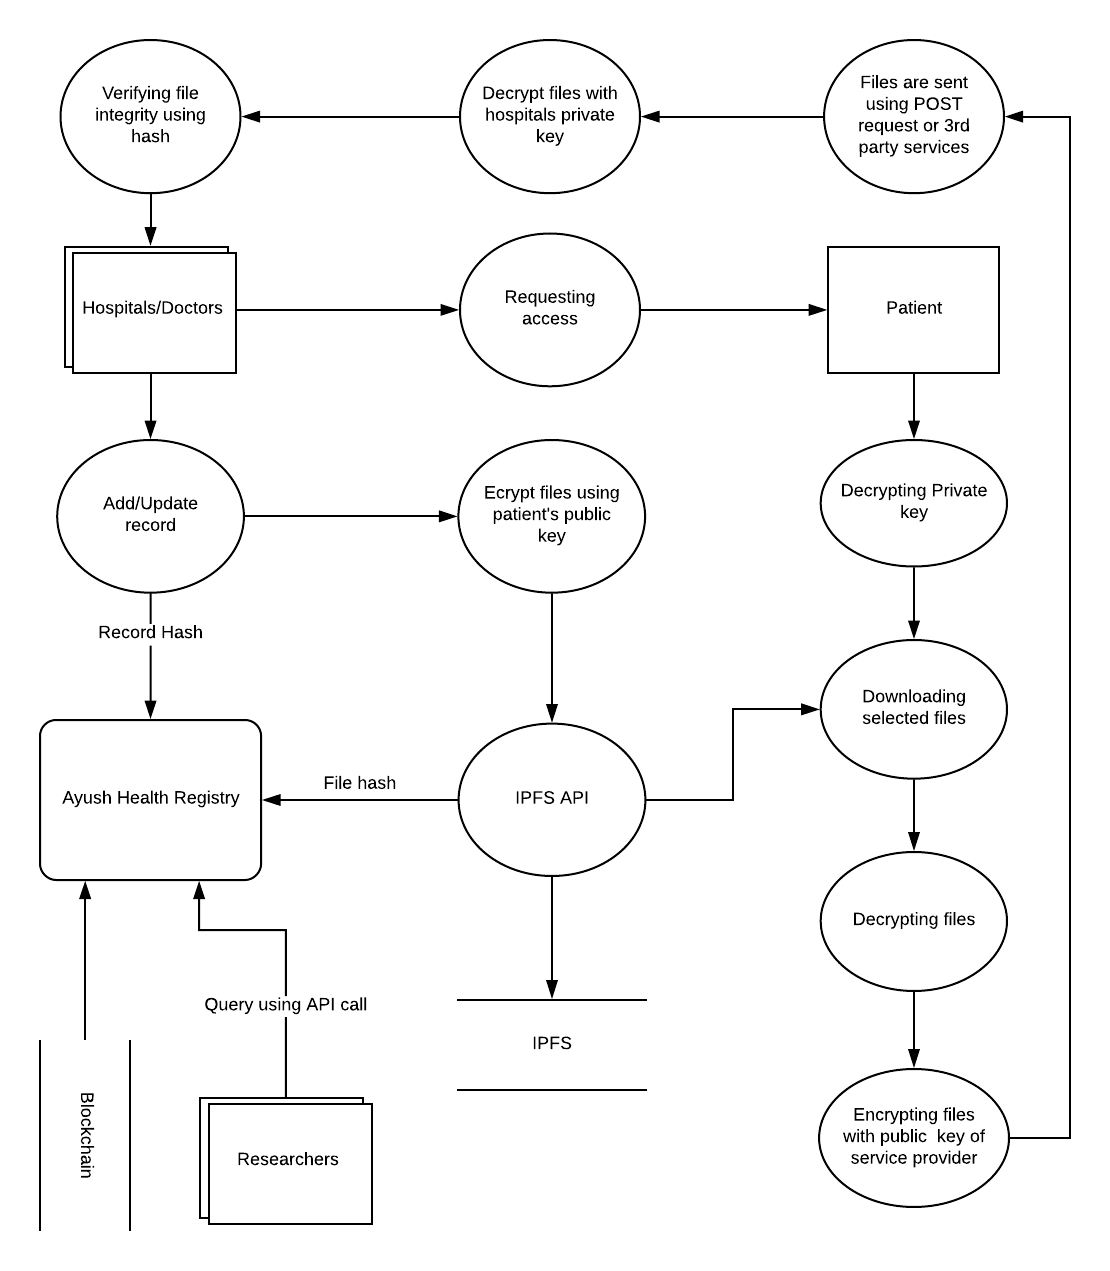
\includegraphics[scale=0.9]{DFD2.png}
        \caption{Level 2 DFD}
        \label{fig:my_label}
    \end{figure}
        

\section{Flow Charts}   

    \begin{figure}[h!]
        \centering
        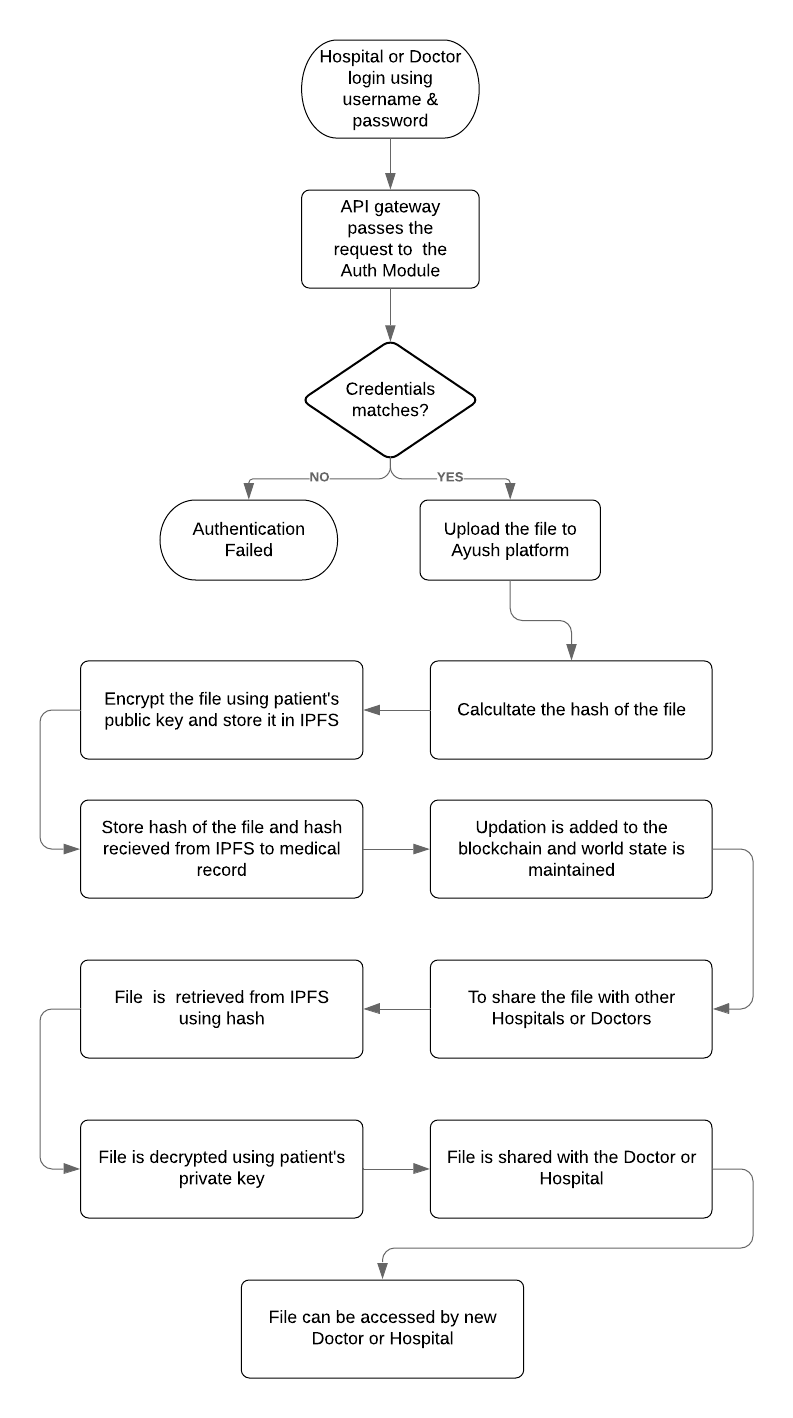
\includegraphics[scale=0.8]{F1.png}
        \caption{User Creation}
        \label{fig:my_label}
    \end{figure}
    
    \begin{figure}[h!]
        \centering
        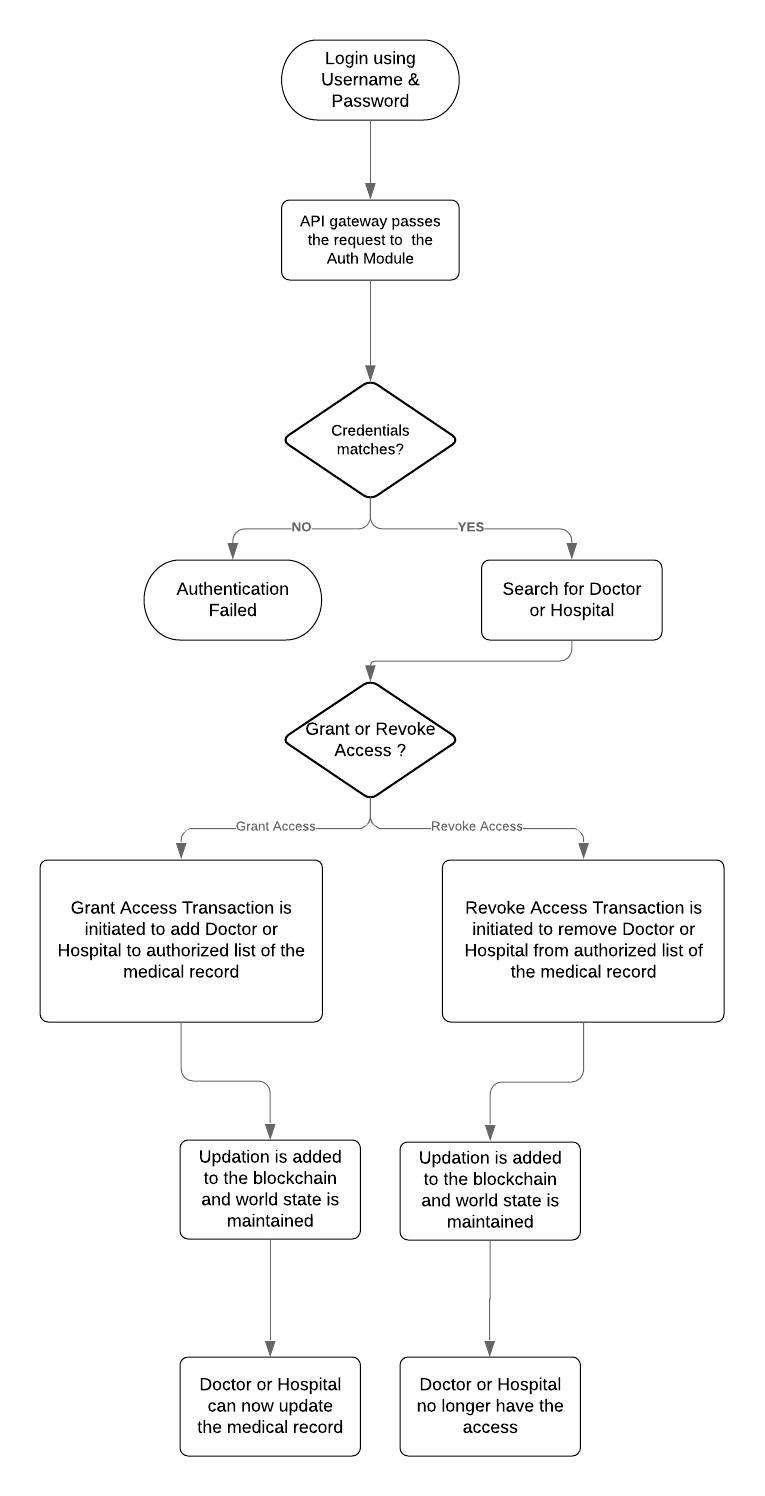
\includegraphics[scale=0.8]{F2.png}
        \caption{File Creation}
        \label{fig:my_label}
    \end{figure}
    
    \begin{figure}[h!]
        \centering
        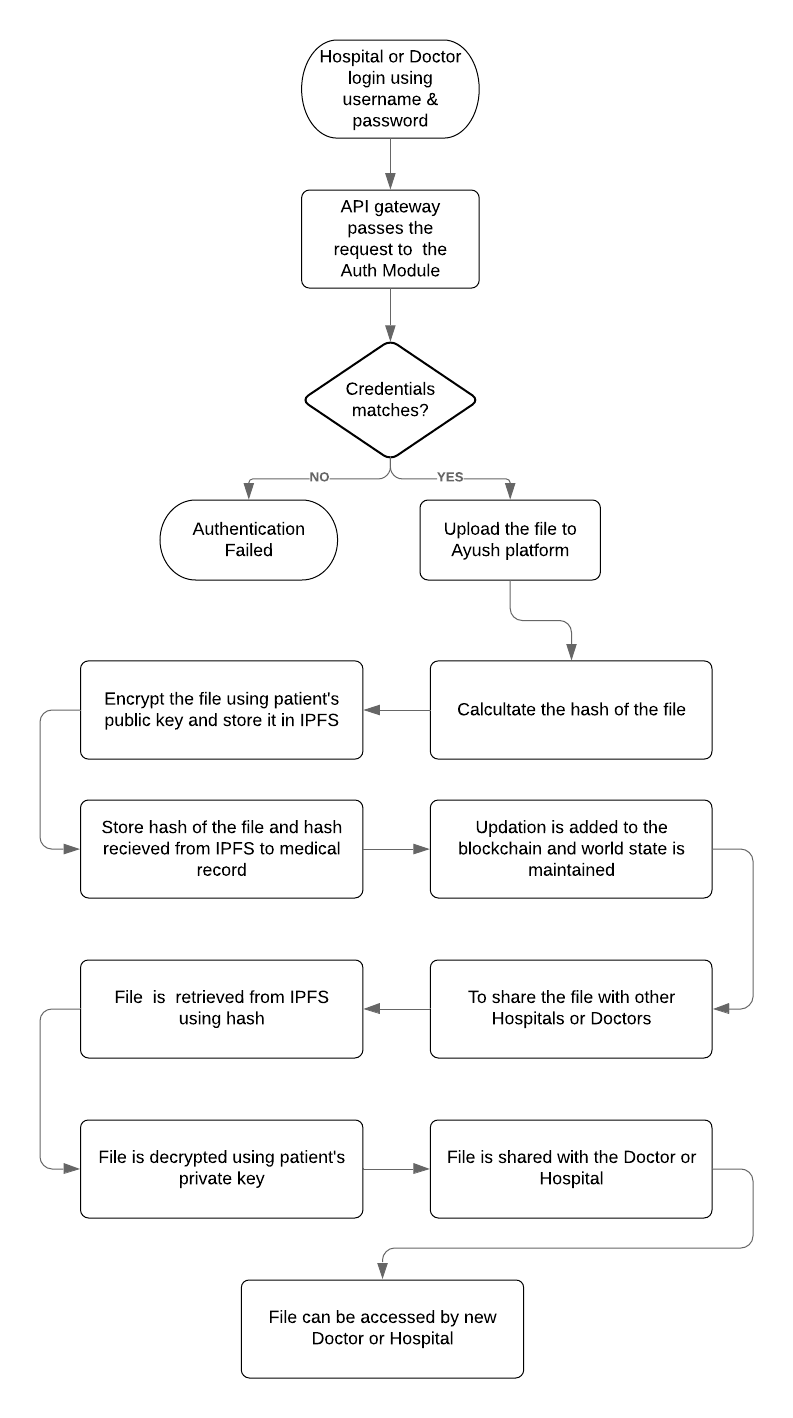
\includegraphics[scale=0.8]{F1.png}
        \caption{Record Sharing}
        \label{fig:my_label}
    \end{figure}
    
   \section{Prototype Design} 
   \subsection{Ayush Home Page}
            \begin{figure}[h!]
        \centering
        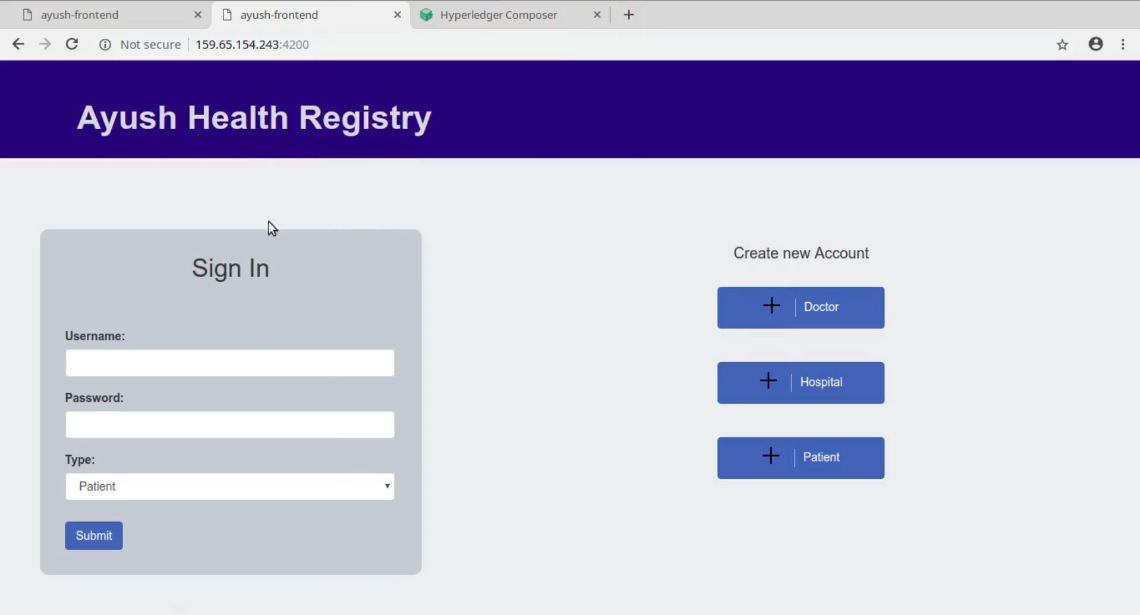
\includegraphics[scale=0.3]{proto1.png}
        \caption{Ayush Home Page}
        \label{fig:my_label}
    \end{figure}
    This screen has 2 options :
    \begin{enumerate}
        \item Sign In
        \item Create New Account
    \end{enumerate}
    \subsubsection{Sign In}
    It has 3 fields
    \begin{enumerate}
        \item Username : Unique Identifier used to identify a user
        \item Password : Secret owned by the user
        \item Type of User : Patient/Doctor/Hospital
    \end{enumerate}
    
    \subsubsection{Create New Account}
    It will help a user to create new account to interact with the Ayush platform.
    
   \newpage 
  \subsection{Patient Dashboard}  
    \begin{figure}
        \centering
        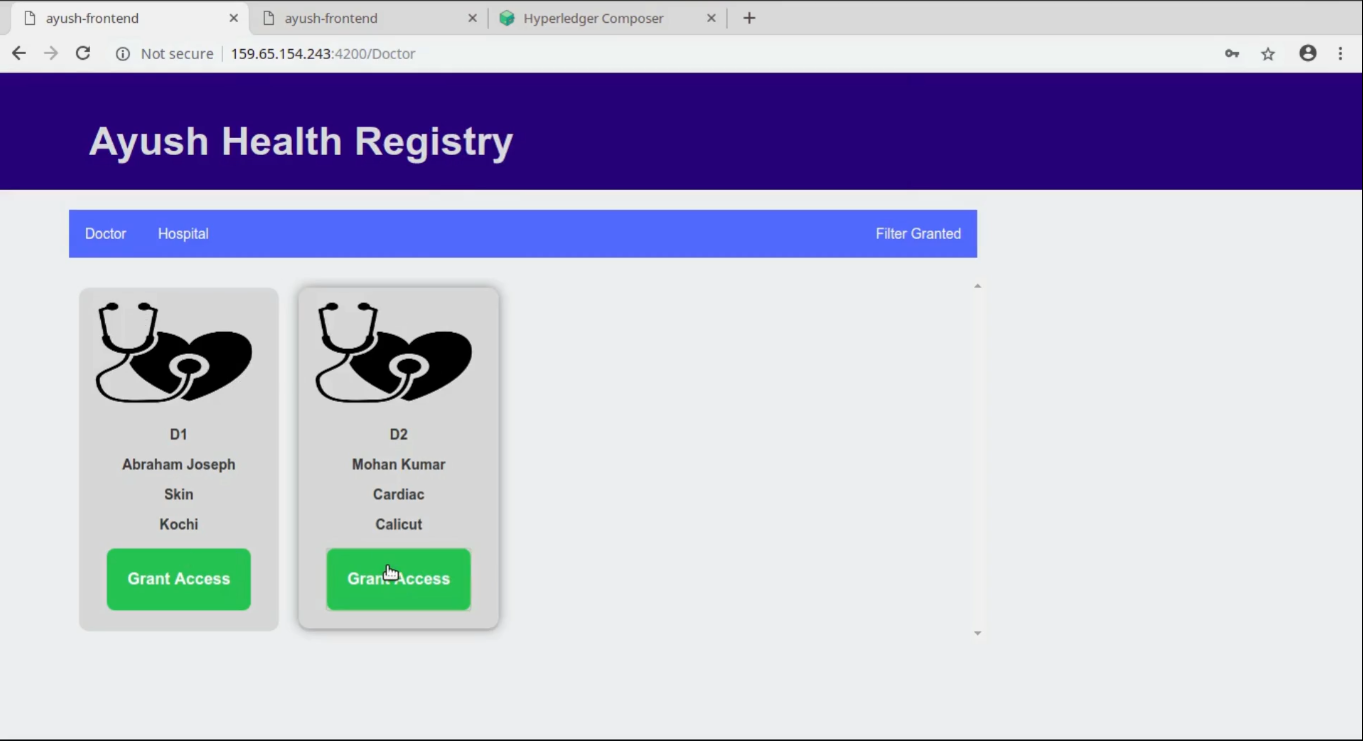
\includegraphics[scale=0.3,width=10cm]{Proto2.png}
        \caption{Patient Dashboard}
        \label{fig:my_label}
    \end{figure}
    Patient Dashboard displays details of doctors and hospitals.Patient can grant or revoke access from doctor and hospital to his medical record. Filtering option is available. 
    \begin{figure}
        \centering
        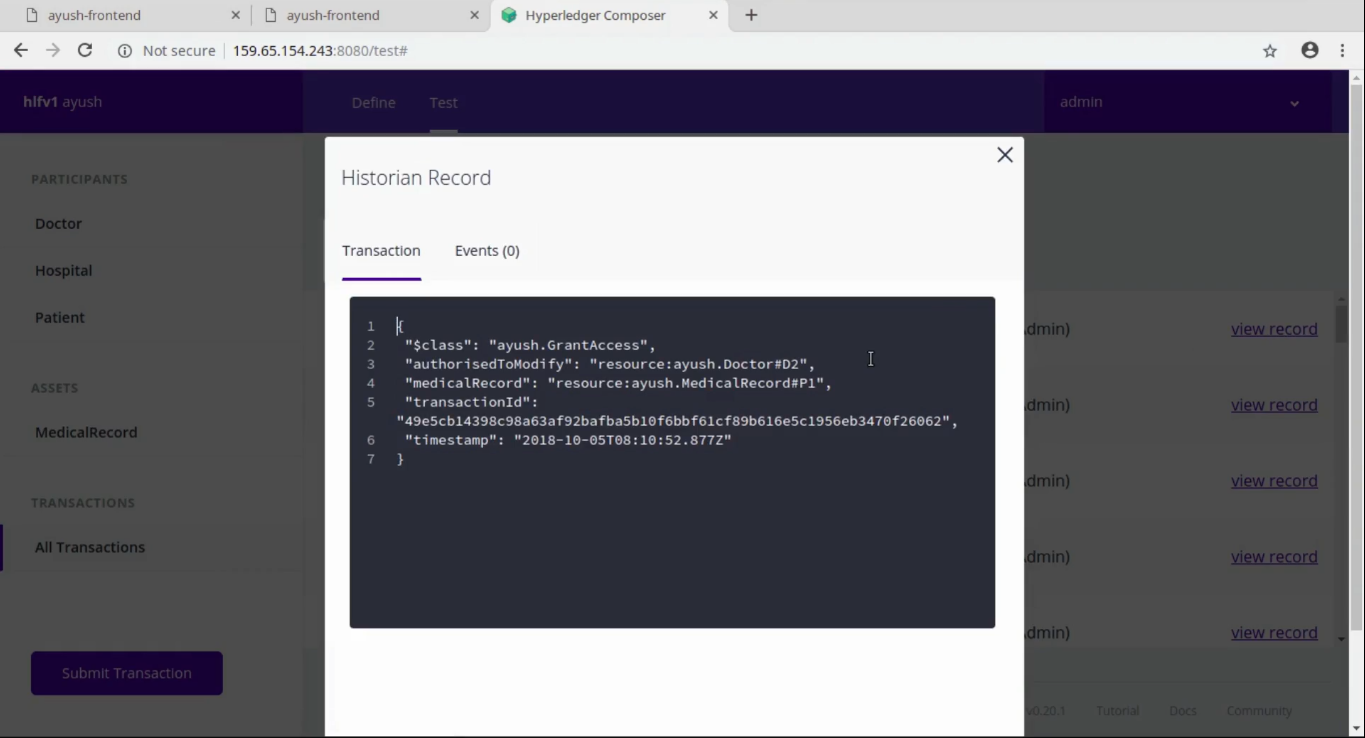
\includegraphics[scale=0.3,width=10cm]{Proto3.png}
        \caption{Prototype Design}
        \label{fig:my_label}
    \end{figure}
    \begin{figure}
        \centering
        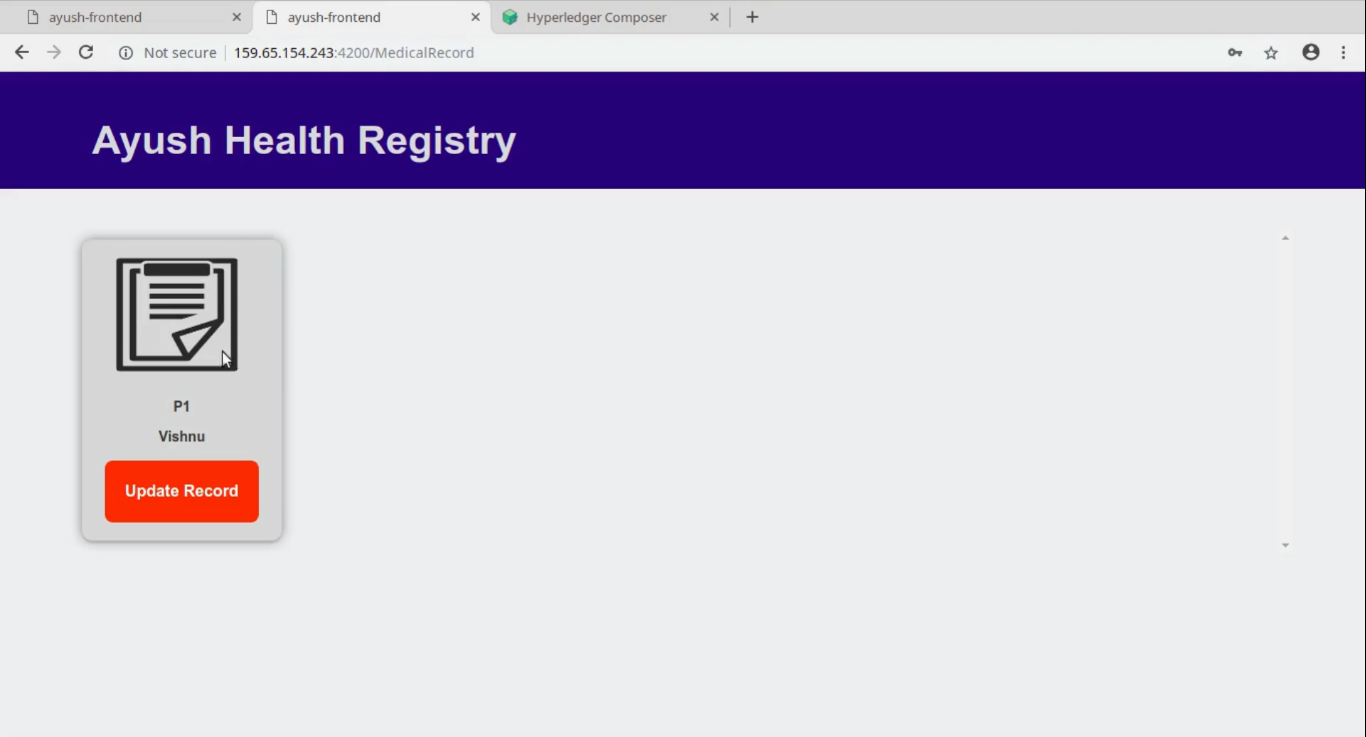
\includegraphics[scale=0.3,width=10cm]{Proto4.png}
        \caption{Prototype Design}
        \label{fig:my_label}
    \end{figure}
    \begin{figure}
        \centering
        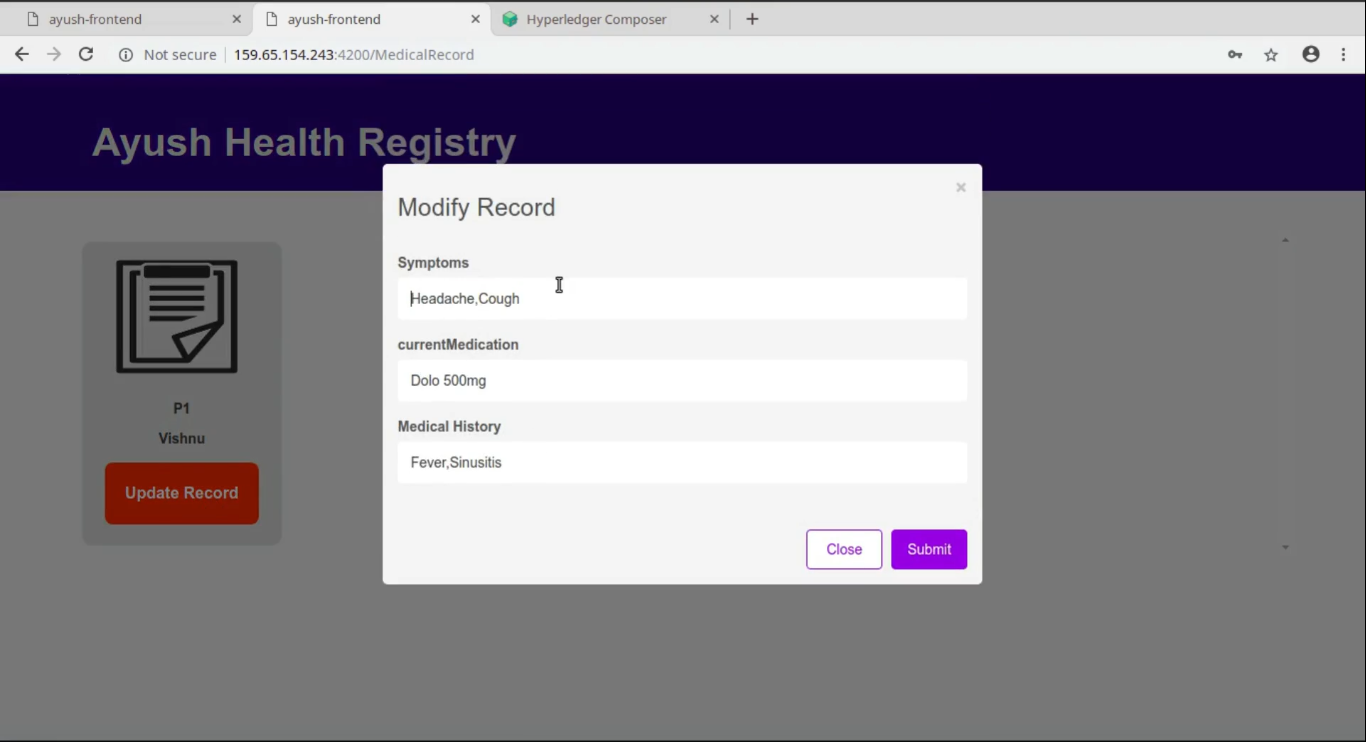
\includegraphics[scale=0.3,width=10cm]{Proto5.png}
        \caption{Prototype Design}
        \label{fig:my_label}
    \end{figure}
    \begin{figure}
        \centering
        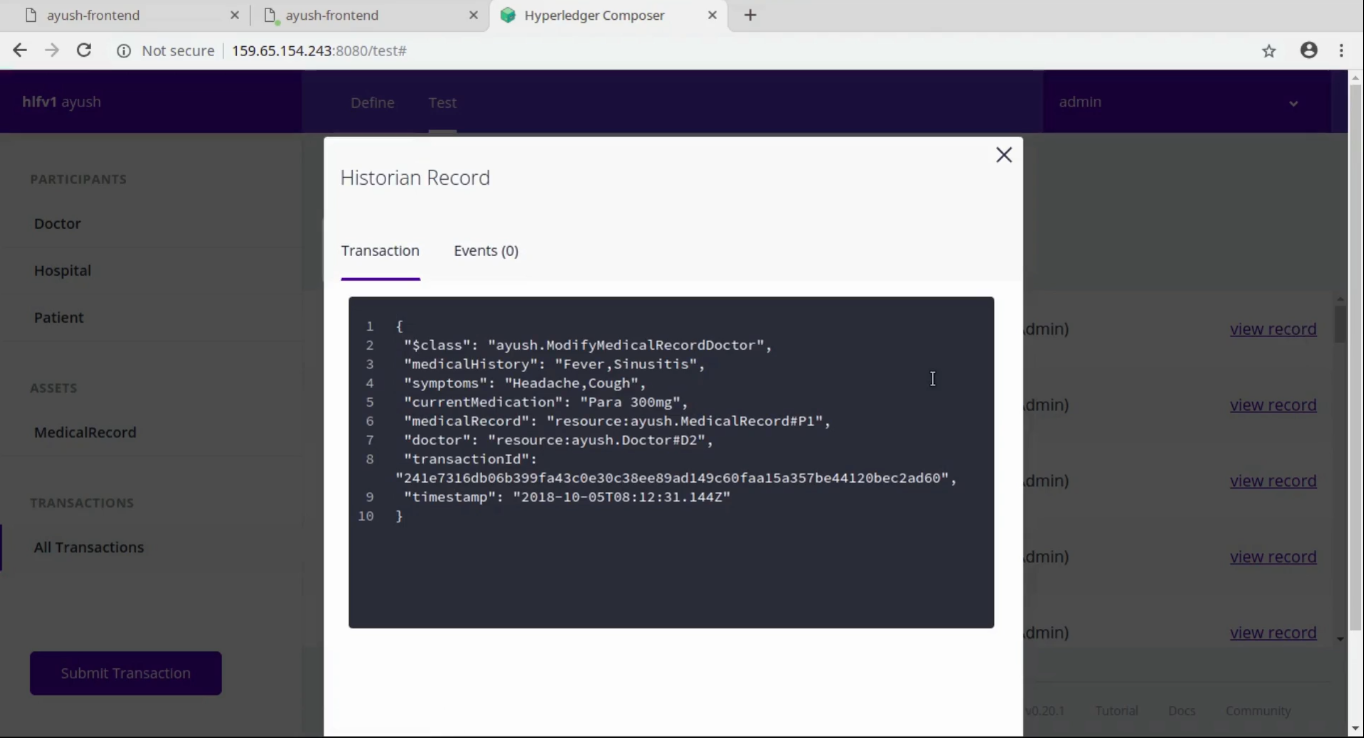
\includegraphics[scale=0.3,width=10cm]{Proto6.png}
        \caption{Prototype Design}
        \label{fig:my_label}
    \end{figure}
\chapter{Hardware and Software Requirements}
        \section{Hardware Requirements}
                \begin{itemize}
                    \item Intel i5 processor
                    \item RAM 8 GB
                \end{itemize}
        \section{Software Requirements}  
                \subsubsection{Operating System}
                            \begin{itemize}
                                \item Ubuntu / Linux
                            \end{itemize} 
                \subsection{Programming Languages}
                            \begin{itemize}
                                \item Bash
                                \item Nodejs
                                \item HTML, CSS, JavaScript
                                \item Typescript
                            \end{itemize}
                 \subsection{Libraries}       
                                \begin{itemize}
                                    \item Hyperledger Fabric
                                \end{itemize}
                \subsection{Data Storage Mechanism}     
                                \begin{itemize}
                                    \item IPFS
                                \end{itemize}
                    
\chapter{Scheduling}
\section{Time Schedule}
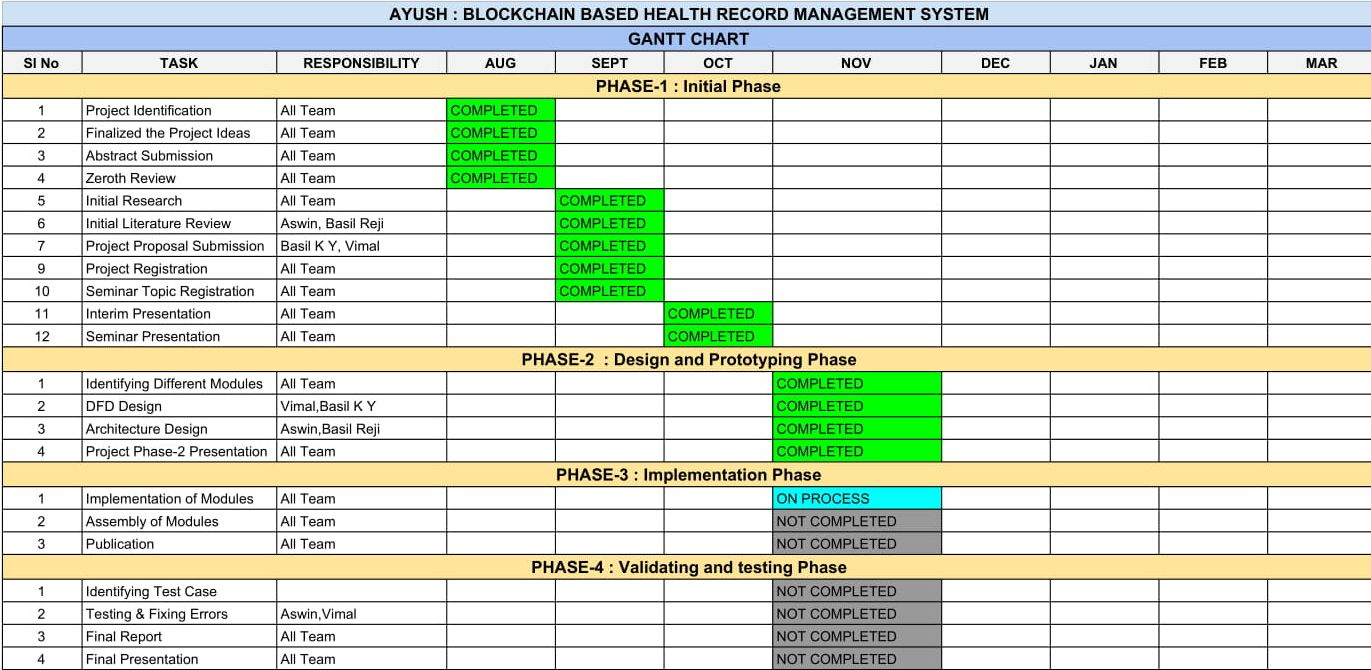
\includegraphics[width=15cm]{Chart.jpeg}\newline
\chapter{Conclusion}
           We are living in a world where data is considered to be the next fuel, also we know how much
value the data is.  We need a patient health record management system to provide more transparency over patient’s past health history, easier data sharing between hospitals and data analytics possibilities while considering the privacy concerns of patients. Using emerging block-chain technology we can create a transparent patient-centric record system. 



%========================== REFERENCES =========================%

\begin{thebibliography}{999}

\addcontentsline{toc}{chapter}{References}


\bibitem{1} \textquotedblleft  Secure Attribute-Based Signature Scheme With Multiple Authorities for Blockchain in Electronic Health Records Systems\textquotedblright, \textit 
{Available: https://ieeexplore.ieee.org/document/8279429/}


\bibitem{2} \textquotedblleft Blockchain: Solving the privacy and research availability tradeoff for EHR data: A new disruptive technology in health data management\textquotedblright 
\textit{Available: http://https://ieeexplore.ieee.org/document/8263269/}

\bibitem{3} \textquotedblleft Using Blockchain for Medical Data Access and Permission Management\textquotedblright 
\textit{Available: https://ieeexplore.ieee.org/document/7573685/}


\bibitem{4}G. Zyskind, O. Nathan and A. '. Pentland, "Decentralizing Privacy: Using Blockchain to Protect Personal Data," 2015 IEEE Security and Privacy Workshops, San Jose, CA, 2015, pp. 180-184.
URL: http://ieeexplore.ieee.org/stamp/stamp.jsp?tp=arnumber=7163223isnumber=7163193

\bibitem{5}Securing Mobile Health Data Transmissions with Blockchain Technology
URL : https://innovate.ieee.org/innovation-spotlight/blockchain-mobile-health-data-wearables/

\bibitem{6}Blockchain: 
Opportunities for Health Care 
URL : https://www2.deloitte.com/content\\/dam/Deloitte/us/Documents/public-sector/us-blockchain-opportunities-for-health-care.pdf

\bibitem{7} 
M. Mettler, "Blockchain technology in healthcare: The revolution starts here," 2016 IEEE 18th International Conference on e-Health Networking, Applications and Services (Healthcom), Munich, 2016, pp. 1-3.
URL: http://ieeexplore.ieee.org/stamp/stamp.jsp?tp=arnumber=7749510isnumber=7749413

\bibitem{8} Ariel Ekblaw, Asaph Azaria , John D. Halamka, MD, Andrew Lippman, \textquotedblleft A Case Study for Blockchain in Healthcare:
“MedRec” prototype for electronic health records and medical research data\textquotedblright, \textit{MIT Media Lab,Beth Israel Deaconess Medical Center}, August,2016.

\end{thebibliography}
 

\end{document}
